\documentclass[a4paper,oneside,11pt]{article}
\usepackage{a4wide,graphicx,fancyhdr,amsmath,amssymb}

%-------- Macros and Definitions --------%

\setlength\headheight{20pt}
\addtolength\topmargin{-10pt}
\addtolength\footskip{20pt}

\newcommand{\subject}{2IO70 embedded systems}

\newcommand{\N}{\mathbb{N}}
\newcommand{\ch}{\mathcal{CH}}

\newcommand{\naam}{Reinhard Heinrich Bertram Vinzenz Freiherr von Pelden genannt Cloudt zu Lauersfort und Impel}

\fancypagestyle{plain}{%
\fancyhf{}
\fancyhead[LO,RE]{\sffamily\bfseries\large technische universiteit eindhoven}
\fancyhead[RO,LE]{\sffamily\bfseries\large \subject}
\fancyfoot[LO,RE]{\sffamily\bfseries\large department of mathematics and computer science}
\fancyfoot[RO,LE]{\sffamily\bfseries\thepage}
\renewcommand{\headrulewidth}{0pt}
\renewcommand{\footrulewidth}{0pt}
}

\pagestyle{fancy}
\fancyhf{}
\fancyhead[RO,LE]{\sffamily\bfseries\large technische universiteit eindhoven}
\fancyhead[LO,RE]{\sffamily\bfseries\large \subject}
\fancyfoot[LO,RE]{\sffamily\bfseries\large department of mathematics and computer science}
\fancyfoot[RO,LE]{\sffamily\bfseries\thepage}
\renewcommand{\headrulewidth}{1pt}
\renewcommand{\footrulewidth}{0pt}

\usepackage[margin=1in]{geometry}
\usepackage{float}
\usepackage{subcaption}
\usepackage{graphicx}

%-------- Title --------%

\title{\vspace{-\baselineskip}\sffamily\bfseries Software Specification}
\author{
	\makebox[.25\linewidth]{Sergio van Amerongen}\\0952200 \and
	\makebox[.25\linewidth]{Stefan Cloudt}\\0940775 \and
	\makebox[.25\linewidth]{Daan de Graaf}\\0956112 \and
	\makebox[.25\linewidth]{Robert van Lente}\\0953343 \and
	\makebox[.25\linewidth]{Tom Peters}\\0948730 \and
	\makebox[.25\linewidth]{Berrie Trippe}\\0948147 
	\and \makebox[.75\linewidth]{\textbf{Responsible:}} \and
	Tom Peters\\ \tt{t.peters@student.tue.nl}
}
\date{\today}

%-------- Document --------%

\begin{document}
\maketitle

\section{Introduction}
After having designed the machine, we are able to specify how our software should behave. We do this by describing the software in a state machine with abstract states. This state machine also implements the different operation modes. After this we characterise the distinct inputs and outputs. We will convert the state diagram into a working UPPAAL model and explain the working systems in detail. Finally we explain the verification of our model. This chapter is called the software specification.

\section{Operation modes}
The gyroscope can be quite a bottleneck in the sorting process, as it is rather slow. If we want to sort very fast, we should skip the input from the gyroscope and sort the discs immediately after each other. Therefore, we want to implement 2 modes: a fast mode in which we don’t check for input from the gyroscope and thus don’t check if the disc actually reaches the tray, and a slower safe mode, where we check for input from the gyroscope and we can make sure that discs do reach the tray. Besides this, we want to make an additional incremental mode for debug purposes, in which the user has to press a button for the machine to sort the next disc.

\subsection{Fast mode}
The machine starts in a resting state. If the Start/Pause button is pressed in this state, the machine should go to the read color state. In this state, the machine checks which color disc is present on top of the light sensor. There are four different transitions the machine can make at this point, depended on the detected colour. If the machine is black or white, it should go to a respective state in which the motor is rotated accordingly. When the motor has finished moving, the machine simply returns to the read color state. The machine can be paused by pressing the Start/Pause button anytime during the sorting process. The machine then goes to a paused state as soon as it enters the read color state and waits for the Start/Pause again to return to the checking process.

\newpage

\subsection{Safe mode}
The safe mode is exactly the same as the fast mode, with a few additional safety checks. This means that it has the same assumptions according to the input. There is still an arrow from every state except the initial state to the abort state for when the ABORT button is pressed. There are two additional states. One for each colour, black or white. After the motor is finished turning, it enters a state in which it waits for input from the gyroscope (G), which can indicate a disc that felt to the right (R) or to the left (L). When the input is correct, it goes to the state in which the colour is checked. When the input is wrong (Exception) (wrong side, no input at all after a while), the machine goes to the abort state.
\subsection{Incremental mode}
The incremental mode is again almost the same as the safe mode, so again the same assumptions about the input and the state machine, but now there is 1 extra state between the ingoing arrows to the state in which the colour is checked. In this state, the machine waits for a press on a button, the START/STOP button (S/P) to continue. If that button is pressed, it goes to the state in which the colour is checked. All the ingoing arrow that were going to the colour-check state are now going to the wait-for-button-press state. There is 1 exception for this. From the resting state, you go to the colour-check state immediately after a press on the button. It would be silly if you would have to press that button twice for something to happen.

\section{Signals}
\subsection{Inputs:}
\subsubsection{Color c:} The input from the sensor with the following possible values: "N", "W", "B" and "U". The value "N" implies that no disk has been detected in front of the colour sensor. The value "W" implies that a white coloured disk is in front of the sensor. The value "B" implies that a black disk is in front of the sensor. Finally a value "U" means that an unknown disc is in front of the sensor.
\subsubsection{Motor M:} The input from the motor can be that it is jammed, “J”, or that it is finished, “F”. We use these inputs as a method to detect if we can go to the next state, or to detect if there is a possible error.
\subsubsection{Abort A:} This signal is high when the abort button has been pressed. This signal indicates that the machine should be halted nearly instantaneously and that the machine should enter the Abort state.
\subsubsection{Reset R:} This signal is high when the Reset button is pressed. The signal will be used to bring the machine back in its resting state and reset all the statistics about the current sorting operation.
\subsubsection{Start/Pause S/P:} This signal is high when the Start/Pause button is pressed. This signal will be used to start and pause the operation of the machine, depending on its current state.
\paragraph{Gyroscope G:} This signal might have three values "L", "R" and "S". "L" indicates that gyroscope is left, "R" indicates that the gyroscope is right and "S" indicates that the gyroscope is stable.

\subsection{Outputs}
\subsubsection{Colour Sensor CS:} Whether the colour sensor is currently reading the sensor values. In order to read the values, a light from within the sensor has to be activated in order for the detection to work. This means that this light is an output for the machine. While the light is activated, the sensor is constantly reading the sensor values, but we only read it in certain situations. The colour sensor is only active while the machine is in the operating state and is therefore disabled in the Resting state, Abort state, Finished state and the Paused state.
\subsubsection{Motor M:} This signal has three possible values "L", "R" and "O". Where "L" is the motor moving to the left for 120 degrees, "R" is the motor moving to the right for 120 degrees, "O" is the motor turned off. The sorting arm moves, depending on the colour read.
\subsubsection{LED Active E:} The EV3 controller brick has a built-in LED behind the buttons that we can use to give feedback to the user. We can specify the flashing pattern from a limited set of patterns and we can specify the colour. The LED will emit a constant green colour while the machine is in the Finished state. The LED will flash in red while it is in the Abort state. The LED will flash orange when it is in a warning state.
\subsubsection{Sound:} The brick also features a built-in speaker which we can use to give even more feedback to the user. We will use this speaker to let the user now what happens in the machine. So when there is an error, the machine will sound an error. When the machine finishes sorting it will play tiroler music.

\section{State Machine}
\begin{figure}[H]
	\centering
	\includegraphics[width=140mm]{statemachine}
	\caption{This state machine defines the behaviour of the software. The three modes of our machine have been embedded into the figure. Black coloured transitions are done in all modes.}
\end{figure}
We have indicated the transitions for specific modes using a colour coding. Green transitions only apply to the fast mode. Red transitions only apply to the incremental mode. Blue transitions only apply to the safe mode. 

All symbols are inputs or outputs defined in the next chapter. However some symbols are not input or output but something else, these are documented here:

\begin{figure}[H]
\begin{tabular}{|l|l|}
\hline
\textbf{Symbol} & \textbf{Description} \\
\hline
PS & Starts the peripherals in order to be able to use them. This means setting output CS \\
 &  to active and M=O \\
PR & Resets the peripherals to turn them off, sets the CS to non active and M=O \\
TS & Starts a timer which increments variable $t$ at a fixed time rate \\
TR & Resets the timer by setting $t$ to 0\\
$t$ & The variable containing the current timer value \\
$tdmax$ & The maximum timer value after which it is decided that a disk was lost \\
$tavg$ & The average time of a disk to get in the basket \\
$tgmax$ & The maximum time it should take to stabilize the gyroscope \\
$paused$ & Variable indicating if the machine should go into the paused state or not \\
$reset$ & Variable indicating if the machine should go into the reset state or not \\
\hline
\end{tabular}
\end{figure}

\section{UPPAAL model}
An UPPAAL model consist of multiple systems that communicate over several channels. The systems in our UPPAAL model are Reinhard, our main system, along with several other peripheral systems.

\begin{figure}[H]
	\centering
	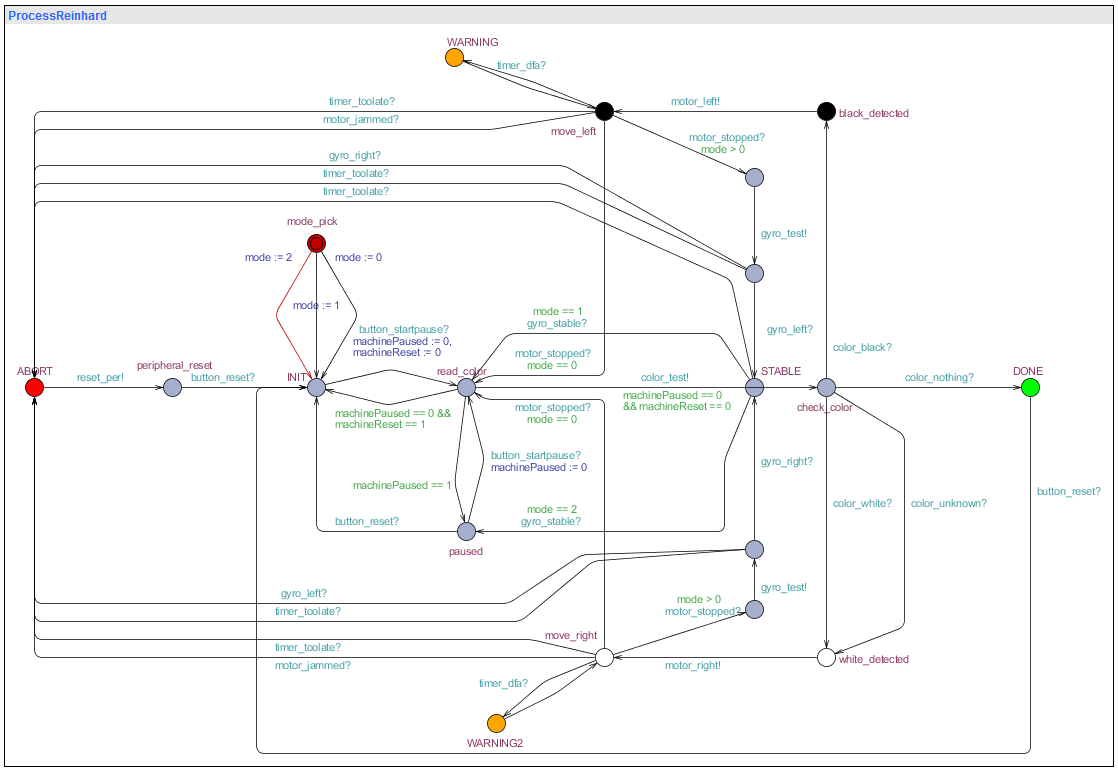
\includegraphics[width=150mm]{mainprocess}
	\caption{This state machine defines the behaviour of the software. The three modes of our machine have been embedded into the figure. Black coloured transitions are done in all modes.}
\end{figure}

\subsection{Main process}
\subsubsection{Choosing the mode}
The initial state is mode\_pick, which is not present in the state machine. In this mode one of the three operation modes is chosen. This is important for the verification process, because the UPPAAL model uses an internal variable to store the mode, whereas the state machine indicates the different modes with colours. If it is not possible to set this variable in the model itself, the verification process will only verify if a query holds for one mode.

\subsubsection{Initialiation}
Upon choosing a mode, we enter the state INIT, which is equivalent to the initial state in the state machine. Here, the model waits for the button\_startpause signal from ProcessButtons. Also, it sets the machinePaused and machineReset variable to 0, which ensures that the model does not immediately pause or reset.

\subsubsection{Reading colours}
Upon leaving the INIT state we enter the read\_color state(read in the state machine). Whenever the machinePaused variable is 1 in the read\_color state, the model goes to the paused state. If the machineReset variable is 1, the machine returns to the INIT state, but this has the lower priority. If both of these are 0, the color\_test signal is send and the model transitions to the check\_color state.  In the check\_color state it waits for a signal of the ColorSensor system depending on whether there is a disc and which colour the disc has. Depending on the colour, it goes to one of two parts of the main system, one for each distinct colour (black or white). We will describe one of these parts as they are mirrored. Upon receiving the signal of a colour, the model transitions to a detected state. Here, it sends a signal to ProcessMotor to start moving in the appropriate direction and goes into a move state. The transition the model makes here is dependent on the mode variable.

\subsubsection{Check sequence}
If mode is not 0, indicating that the system is in the safe or incremental mode, it will add a check sequence using the gyroscope. After the signal from the motor is received that it has stopped, the main system will send a test signal to the GyroSensor waiting for a signal back. If the correct signal is received back, indicating that the disc has arrived in the correct tray, it will return to read\_color state. If mode is 0, indicating that the system is in fast mode, this check is skipped and the model returns to the read\_color state from the move state as soon as it receives the motor\_stopped signal from ProcessMotor.

\subsubsection{Finishing up}
When the model receives the color\_nothing signal from ProcessColorSensor, the machine is finished and the model goes to the DONE state. Here it waits for the button\_reset signal and returns to the initial state.

\subsubsection{Exceptions}
In our machine design is it specified that there is an ABORT button present that will stop the whole machine almost immediately. However, we have chosen not to include the abort button in our UPPAAL model as a possible transition for every state because this would be rather cumbersome and just a small implementation. We have however chosen to include possible exceptions such as a jammed motor or a signal that has not arrived in decent time. These transitions will lead the system into the ABORT state. In this state the process waits for the reset button to give a signal, after which it will reset the other processes and return to the intitial state. Note that it is not required to actually reset the gyroscope in the actual machine, just in the UPPAAL model. Non-fatal exceptions are also represented in the model. Deviating average detection time is represented in the states WARNING and WARNING2, which the model reaches when the timer\_dfa is send from ProcessTimer. Process ColorSensor can also send a color\_unknown signal, which sends the machine to WARNING3. These warning states simply return to the state they were detected in and let the model continue.

\subsection{Subprocesses}
The following are all subprocesses that the main process depends on:

\subsubsection{ProcessColorSensor} waits for the $color\_test$ signal. It can then send four different signals: $color\_black$, $color\_white$, $color\_unknown$, and $color\_nothing$.

\subsubsection{ProcessMotor} waits for the $motor\_left$ or $motor\_right$ signal and moves to the respective state. From there, it can send either a $motor\_stopped$ or a $motor\_jammed$ signal. It also listens for a $reset\_per$ signal, after which it returns to the initial state.

\subsubsection{ProcessGyroSensor} waits for the $gyro\_test$ signal from the main process. It can then send the following signals: $gyro\_stable$, $gyro\_left$ and $gyro\_right$. If either $gyro\_left$ or $gyro\_right$ is send, the machine goes to an additional state where it is able to send a $gyro\_stable$ signal, indicating that the gyroscope has returned to its initial position. The process also listens for the $reset\_per$ signal, for resetting purposes.

\subsubsection{ProcessButtons} is continuously able to send button signals. This simulates that any button can be pressed at any time, which is necessary for the verifier to check all possible transitions. 

\subsubsection{ProcessTimer} works the same as ProcessButtons, but with signals that an internal timer would send if it detected one of the errors.

\subsubsection{ProcessPauseListener} and \textbf{ProcessResetListener} continuously listen to the $button\_startpause$ and $button\_reset$ signals from ProcessButtons. When they detect the respective signals, they set the respective variables to 1 to alert the main process that the button is pressed.

\begin{figure}
\centering
\begin{subfigure}{0.1\textwidth}
\centering
\includegraphics[height=55mm]{processcolorsensor}
\caption{Colour sensor}
\end{subfigure}
\hfill
\begin{subfigure}{0.3\textwidth}
\centering
\includegraphics[height=55mm]{processmotor}
\caption{Motor}
\end{subfigure}
\hfill
\begin{subfigure}{0.3\textwidth}
\centering
\includegraphics[height=55mm]{processgyrosensor}
\caption{Gyroscope}
\end{subfigure}

\begin{subfigure}{0.45\textwidth}
\centering
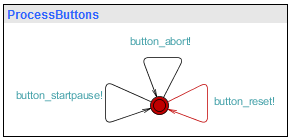
\includegraphics[height=30mm]{processbuttons}
\caption{Buttons}
\end{subfigure}
\hfill
\begin{subfigure}{0.45\textwidth}
\centering
\includegraphics[height=30mm]{processtimer}
\caption{Colour sensor}
\end{subfigure}

\begin{subfigure}{0.45\textwidth}
\centering
\includegraphics[height=50mm]{processpauselistener}
\caption{Pause listener}
\end{subfigure}
\hfill
\begin{subfigure}{0.45\textwidth}
\centering
\includegraphics[height=50mm]{processresetlistener}
\caption{Reset listener}
\end{subfigure}
\caption{Subprocesses}
\end{figure}

\section{Verification}
The main reason for recreating the state machine in UPPAAL was to allow extensive verification of the model. With UPPAAL we can verify the events like deadlock will never occur. The UPPAAL query language is a minimalistic but functional language to specify these properties. We use the following queries to verify our model:

\subsubsection{Abort state reachability}
Query: E$<>$ ProcessReinhard.ABORT \\
Description: There exists a path where the system reaches the ABORT state.\\
We want to ensure that the machine halts in case of a fatal error. This check ensures that it is theoretically possible for a fatal error to occur and jump to the ABORT state.

\subsubsection{Peripheral reset}
Query: A[] (ProcessReinhard.paused or ProcessReinhard.INIT) imply (ProcessMotor.INIT and ProcessGyroSensor.INIT) \\
Description: Whenever the system is in the paused or initialisation state, the motor and gyro sensor must be in their initial state. \\
The goal is this check is twofold: We want to ensure that all peripherals are idle when the machine is in the paused state or has not yet started, and we have to be certain that after reaching the ABORT state, all peripherals are correctly reset. If we would leave the gyroscope in its left or right state, we would cause deadlock in the next cycle. Worse still, leaving the motor running after an ABORT could harm to machine.

\subsubsection{Full speed independent of gyroscope}
Query: A[] mode == 0 imply ProcessGyroSensor.INIT \\
Description: When in full speed mode, the system must leave the gyroscope in its initial state. \\
Full speed mode is supposed to ignore the gyroscope to speed up the sorting process. Here we check if the machine correctly uses the mode setting.

\subsubsection{DONE state reachability}
Query: E$<>$ ProcessReinhard.DONE \\
Description: There exists a path where the system reaches the ABORT state \\
This check ensures that the machine can eventually finish the sorting process.

\subsubsection{Machine pause justify}
Query: A[] ((ProcessReinhard.paused and mode != 2) imply machinePaused==1) \\
Description: Whenever the system is in the paused state and not in incremental mode, machinePaused must be set to 1. \\
Verifies that in the full speed and safe modes, the machine only reaches the paused state when the pause button was pressed beforehand.

\subsubsection{Valid mode specified}
Query: A[] mode==0 or mode==1 or mode==2 \\
Description: Mode must be one of: full speed, safe or incremental. \\
The mode value must be valid.

\subsubsection{No deadlock}
Query: A[] not deadlock \\
Description: The system never deadlocks in any case \\

\section{Conclusion}
this chapter provided the information about the behaviour of our software. We introduced our state machine diagram which we then implemented in UPPAAL. We clearly explained the working of our systems in UPPAAL and verified our model using this program. This part is used as the basis for the design of the software and is very important.

\end{document}
